
	In its most basic form, a phase locked loop is a phase-based feedback system whose output tracks or maintains a fixed phase relationship to an input signal. As will be shown, such a system is uniquely suited to the task of frequency synthesis, which is the process of generating derivative frequencies from some reference frequency. Given reference and output phase signals $\Phi_{ref}$ and $\Phi_{out}$, a PLL can be modeled as in figure \ref{fig:basic_fb}, with feedforward and feedback networks A(s) and B(s). 
	\begin{figure}[htb!]
		\center\fontfamily{\sfdefault}\selectfont
% XCircuit output "basic_feedback.tex" for LaTeX input from basic_feedback.ps
\def\putbox#1#2#3#4{\makebox[0.00000in][l]{\makebox[#1][l]{}\raisebox{\baselineskip}[0.00000in][0.00000in]{\raisebox{#2}[0.00000in][0.00000in]{\scalebox{#3}{#4}}}}}
\def\rightbox#1{\makebox[0.00000in][r]{#1}}
\def\centbox#1{\makebox[0.00000in]{#1}}
\def\topbox#1{\raisebox{-0.60\baselineskip}[0.00000in][0.00000in]{#1}}
\def\midbox#1{\raisebox{-0.20\baselineskip}[0.00000in][0.00000in]{#1}}
   \scalebox{1}{
   \normalsize
   \parbox{3.61667in}{
   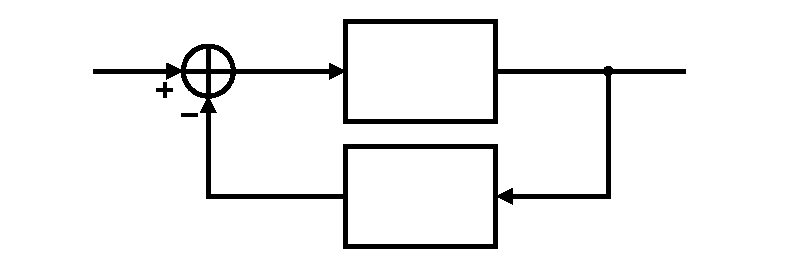
\includegraphics[scale=0.70000]{./figs/basic_feedback.pdf}\\
   % translate x=544 y=496 scale 0.38
   \putbox{1.82000in}{0.85400in}{1.20}{A(s)}%
   \putbox{1.82000in}{0.27300in}{1.20}{B(s)}%
   \putbox{0.44800in}{1.00100in}{1.20}{$\Phi_{ref}$}%
   \putbox{2.84200in}{1.00100in}{1.20}{$\Phi_{out}$}%
   \putbox{1.12000in}{1.00100in}{1.20}{$\Phi_{error}$}%
   } % close 'parbox'
   } % close 'scalebox'
   \vspace{-\baselineskip} % this is not necessary, but looks better
\fontfamily{\rmdefault}\selectfont

		\caption{Basic phase feedback network.}
		\label{fig:basic_fb}
	\end{figure}
	\FloatBarrier
	The closed loop phase response T(s) for $\Phi_{ref}$ to $\Phi_{out}$ is therefore:
	\begin{equation}
		\mathrm{T}(s) = \frac{\Phi_{out}(s)}{\Phi_{ref}(s)} = \frac{A(s)}{1+A(s)B(s)}
	\end{equation}
	A particular case of interest is when B(s) = 1/N, where N is a constant, and the loop gain A(s)B(s) $>>$ 1, the closed loop response is:
	\begin{equation}\label{mult_by_n}
		\frac{\Phi_{out}(s)}{\Phi_{ref}(s)} \approx \frac{A(s)}{A(s)B(s)} = \frac{1}{B(s)} = N
	\end{equation}
	We see that the phase through the PLL is multiplied by a factor of N. If the input phase signal is a sinusoid with frequency $\omega_{ref}$, and likewise the output with $\omega_{out}$, then $\phi_{ref}(t)=\omega_{ref}t$ and $\phi_{out}(t)=\omega_{out}t$. Thus:
	\begin{equation}
		\frac{\Phi_{out}(t)}{\Phi_{ref}(t)} = \frac{\omega_{out}t}{\omega_{ref}t} \approx N \hspace{1em} \rightarrow \hspace{1em} \omega_{out} \approx N\omega_{ref}
	\end{equation}
	Therefore, it is observed that a PLL allows for the generation, i.e. synthesis, of a new frequency from a reference frequency signal. Given a feedback divider ration of 1/N, the PLL multiplies the reference frequency by a factor of N. In the following sections, more advanced models for PLL will be developed, extending the concept introduced here. Specifically, the theory of digital, discrete-time PLLs will be developed and extended from a continuous phase model of a basic PLL.

	\subsection{Continuous PLL Model}
		Although PLLs are practically limited to using discrete-time sampling in real-word hardware, continuous models can still be applied in their analysis and design. Thus a continuous PLL model is developed in this section to aid in the later discussed discretized PLL modeling.

		\subsubsection{PLL Synthesizer architecture}
			The traditional architecture for implementing a PLL frequency synthesizer \cite{Razavi1996DesignOM} is shown in figure \ref{fig:basic_pll}. This basic PLL is comprised of four components: (1) a phase detector, denoted by PD, (2) a loop filter, denoted by H$_{LF}$(s), (3) a voltage controlled oscillator, denoted by VCO, and (4) and phase divider, denoted by "$\div$ N" in the figure. These components are explained in the following sections.
			\begin{figure}[htb!]
				\center\fontfamily{\sfdefault}\selectfont
% XCircuit output "basic_pll.tex" for LaTeX input from basic_pll.ps
\def\putbox#1#2#3#4{\makebox[0.00000in][l]{\makebox[#1][l]{}\raisebox{\baselineskip}[0.00000in][0.00000in]{\raisebox{#2}[0.00000in][0.00000in]{\scalebox{#3}{#4}}}}}
\def\rightbox#1{\makebox[0.00000in][r]{#1}}
\def\centbox#1{\makebox[0.00000in]{#1}}
\def\topbox#1{\raisebox{-0.60\baselineskip}[0.00000in][0.00000in]{#1}}
\def\midbox#1{\raisebox{-0.20\baselineskip}[0.00000in][0.00000in]{#1}}
   \scalebox{1}{
   \normalsize
   \parbox{4.49167in}{
   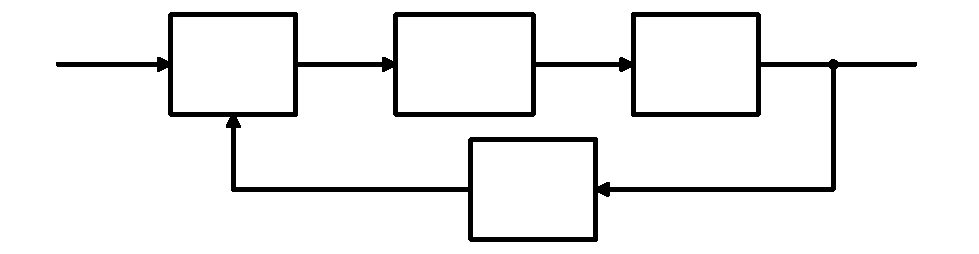
\includegraphics[scale=0.70000]{./figs/basic_pll.pdf}\\
   % translate x=320 y=488 scale 0.38
   \putbox{0.97300in}{0.82600in}{1.20}{PD}%
   \putbox{2.34500in}{0.24500in}{1.20}{$\div$ N}%
   \putbox{0.32900in}{0.97300in}{1.20}{$\Phi_{ref}$}%
   \putbox{3.71700in}{0.97300in}{1.20}{$\Phi_{out}$}%
   \putbox{1.90400in}{0.82600in}{1.20}{H$_{LF}$(s)}%
   \putbox{3.07300in}{0.82600in}{1.20}{VCO}%
   \putbox{1.49800in}{0.39200in}{1.20}{$\Phi_{div}$}%
   \putbox{1.52600in}{0.97300in}{1.20}{$\Phi_e$}%
   \putbox{2.54800in}{0.97300in}{1.20}{V$_{ctrl}$}%
   } % close 'parbox'
   } % close 'scalebox'
   \vspace{-\baselineskip} % this is not necessary, but looks better
\fontfamily{\rmdefault}\selectfont

				\caption{Basic PLL.}
				\label{fig:basic_pll}
			\end{figure}
			\FloatBarrier

		\subsubsection{Divider}
			The phase divider is used as the feedback path in the PLL, where the division modulus N controls the frequency multiplication of the PLL. The tranfer function of the divider is:
			\begin{equation}
				\mathrm{H}_{div}(s) = \frac{\Phi_{div}(s)}{\Phi_{out}(s)} = \frac{1}{\mathrm{N}}
			\end{equation}

			\subsubsection{Phase detector}
			The phase detector is used to measure the phase of the feedback signal (i.e. divider output) in relation to the reference phase, in order to establish a phase error signal $\Phi_e$ used to control the tuning of the PLL.
			\begin{equation}
				\Phi_e(s) = \Phi_{ref}(s) - \Phi_{div}(s)
			\end{equation}

		\subsubsection{Loop Filter}
			The PLL loop filter is used to control the phase-frequency response of PLL, which affects transient PLL behavior, as well as phase noise performance (see section \ref{pn_theory}). As will later be seen, low pass response is desired in a PLL, so the loop filter must be designed accordingly. Generally, this can be designed arbitrarily to have P poles and Z zeros, as such:
			\begin{equation}
				\textnormal{H}_{LF}(s) = \frac{\Sigma_0^Z b_js^j}{\Sigma_0^P a_ks^k}
			\end{equation}
			Rational choice of the loop filter will ensure that the PLL will be stable and minimize steady state phase error. In order to achieve zero steady state error, the loop filter must contain a pole at zero, in other words an integrator. A PLL containing such a pole is classified as a Type II PLL, and a PLL omitting the pole is considered Type I. A logical approach to loop filter design for zero-phase error is to treat it as a PID controller, where:
			\begin{equation}
				\textnormal{H}_{LF}(s) = sK_d + K_p + \frac{K_i}{s} = \frac{K_d}{s}\left(s^2 + s\frac{K_p}{K_d} + \frac{K_i}{K_d}\right)
			\end{equation}
			Such a loop filter contains two zeros and one integrator pole at zero. The gain parameters $K_p, K_i, K_d$ can be tuned to achieve the desired bandwidth and stability for the PLL. The impacts of loop filter design will be further considered in sections \ref{cont_pll_tf}-\ref{other_pid}.
			
		\subsubsection{VCO}
			The voltage controlled oscillator is an oscillator with frequency controlled by an input signal V$_{ctrl}$. The VCO is characterized by its gain $K_{DCO} = \partial f/\partial \textnormal{V}_{ctrl}$, and the nominal oscillation frequency $f_0$. Analyzed in terms of phase, an oscillator can be seen as a time-phase integrator:
			\begin{equation}
				\Phi_{VCO}(t) = \Phi_{out}(t) = \int2\pi(K_{DCO}\textnormal{V}_{ctrl}(t) + f_0)\mathrm{dt}
			\end{equation}
			In s-domain, where frequency offsets will be represented via initial conditions for modeling purposes, the VCO transfer function is therefore:
			\begin{equation}
				\mathrm{H}_{VCO}(s) = \frac{\Phi_{VCO}(s)}{\textnormal{V}_{ctrl}(s)} = \frac{\Phi_{out}(s)}{\textnormal{V}_{ctrl}(s)} = \frac{2\pi K_{DCO}}{s}
			\end{equation}

		\subsubsection{Continuous PLL Transfer function}\label{cont_pll_tf}
			Now that the continuous PLL synthesizer is understood at a component level, the closed loop dynamics of the PLL can be analyzed. First the PLL loop gain is determined:
			\begin{equation}
				\mathrm{L}(s) = \textnormal{H}_{LF}(s)\textnormal{H}_{VCO}(s)\textnormal{H}_{div}(s) = \frac{2\pi K_{VCO}K_d}{\mathrm{N}}\frac{1}{s^2}\left(s^2 + s\frac{K_p}{K_d} + \frac{K_i}{K_d}\right)
			\end{equation}
			With the phase detector as the feedback summation point, the closed loop response of the PLL from reference to output is:
			\begin{align} \label{eq:pid_pll_tf}
				\mathrm{T}(s) = \frac{\Phi_{out}(s)}{\Phi_{ref}(s)} = \frac{2\pi K_{VCO}\left(s^2K_d + sK_p + K_i\right)}{s^2\left(1 + \frac{2\pi K_{VCO}K_d}{\mathrm{N}}\right) + \frac{2\pi K_{VCO}}{\mathrm{N}}\left(sK_p + K_i\right)} = \mathrm{N}\frac{\mathrm{L}(s)}{1 + \mathrm{L}(s)}
			\end{align}
			It should be noted that in the closed loop configuration, this PLL phase transfer function contains two poles and two zeros. This is not a low pass response as desired for a satisfactory PLL phase noise power spectrum, as will later be discussed. In order achieve low pass operation, the derivative term $K_d$ must be set to zero, yielding a PI controller for the loop filter (with one zero and two poles):
			\begin{align} \label{eq:full_pi_pll_tf}
				\mathrm{T}(s) = \frac{\Phi_{out}(s)}{\Phi_{ref}(s)} = \frac{2\pi K_{VCO}\left(sK_p + K_i\right)}{s^2 + \frac{2\pi K_{VCO}}{\mathrm{N}}\left(sK_p + K_i\right)} = \mathrm{N}\frac{\mathrm{L}(s)}{1 + \mathrm{L}(s)} 
			\end{align}
			Steady state zero phase error can be verified by solving the closed loop $\Phi_e(s)$ for s=0:
			\begin{align}
				\left.\Phi_e(s)\right\vert_{s=0} = \left(\Phi_{ref}(0) - \frac{\Phi_{out}(0)}{\mathrm{N}}\right) = \Phi_{ref}(0)\left(1 - \frac{\Phi_{out}(0)}{\mathrm{N}\Phi_{ref}(0)}\right)= \Phi_{ref}(0)\left(1 - \frac{\mathrm{N}}{\mathrm{N}}\right) = 0
			\end{align}

		\subsubsection{PI-loop filter design}
			Given a PI-controller loop filter, which can be optionally represented using a pole at zero and a zero with $\omega_z = K_i/K_p$:
			\begin{equation} \label{eq:pi_pll_tf}
				\textnormal{H}_{LF}(s) = K_p + \frac{K_i}{s}  = \frac{K_i}{s}\left(\frac{s}{\omega_z} + 1\right) 
			\end{equation}
			Selection of (not-necessarily optimal) PI controller gains can be easily derived from overall PLL settling time requirements. Suppose that settling time $t_s$ is defined such that the PLL settles within $\pm \delta$ of the final value for a step input. If the initial and final PLL output frequencies are $f_i$ and $Nf_{ref}$, and settling with $\pm f_{tol}$ is desired,  $\delta = f_{tol}/|f_i - Nf_{ref}|$. Setting time is therefore:
			\begin{equation}
				t_s = -\tau\ln(\delta)
			\end{equation}
			Thus, to find settling time, a value for the PLL time constant $\tau$ must be derived. Rewriting equation \ref{eq:full_pi_pll_tf} with substitutions $\omega_z = K_i/K_p$ and $\mathrm{K} = 2\pi K_{VCO}K_i/\mathrm{N}$:
			\begin{equation} \label{eq:simp_pi_pll_tf}
				\frac{\Phi_{out}(s)}{\Phi_{ref}(s)} = \mathrm{N}\cdot\frac{s\frac{K}{\omega_z} + K }{s^2 + s\frac{K}{\omega_z} + K}
			\end{equation}
			If the second order denominator can be redefined in terms of a natural frequency $\omega_n$ and damping $\zeta$, such that:
			\begin{equation}
				s^2 + s\frac{K}{\omega_z} + K = s^2 + s2\zeta\omega_n + \omega_n^2
			\end{equation}
			It is then found that $\omega_n = \sqrt{K}$, and $\omega_z = \sqrt{K}/2\zeta$. The poles of equation \ref{eq:simp_pi_pll_tf} are then located at s = $\zeta\sqrt{K} \pm \sqrt{K}\sqrt{1-\zeta^2}$.
			The settling time of the PLL will be determined by the real portion of dominant pole of equation \ref{eq:simp_pi_pll_tf}, specifically $\tau = 1/|\min(\Re(\{s_{p1}, s_{p2}\}))|$. Based on the pole-zero plot of figure \ref{fig:pi_pll_pz}, it can be observed that the dominant pole location is maximized with $\zeta=1$. The pole-zero loci orientations are based on increasing $\zeta$ values. According to Razavi \cite{razavi_2017}, $\zeta$ is usually 
			"chosen to be $>\sqrt{2}/2$ or even 1 to avoid excessive ringing."
			\begin{figure}[htb!]
				\center\fontfamily{\sfdefault}\selectfont
% XCircuit output "pi_pz_plot.tex" for LaTeX input from pi_pz_plot.ps
\def\putbox#1#2#3#4{\makebox[0.00000in][l]{\makebox[#1][l]{}\raisebox{\baselineskip}[0.00000in][0.00000in]{\raisebox{#2}[0.00000in][0.00000in]{\scalebox{#3}{#4}}}}}
\def\rightbox#1{\makebox[0.00000in][r]{#1}}
\def\centbox#1{\makebox[0.00000in]{#1}}
\def\topbox#1{\raisebox{-0.60\baselineskip}[0.00000in][0.00000in]{#1}}
\def\midbox#1{\raisebox{-0.20\baselineskip}[0.00000in][0.00000in]{#1}}
   \scalebox{1}{
   \normalsize
   \parbox{4.20000in}{
   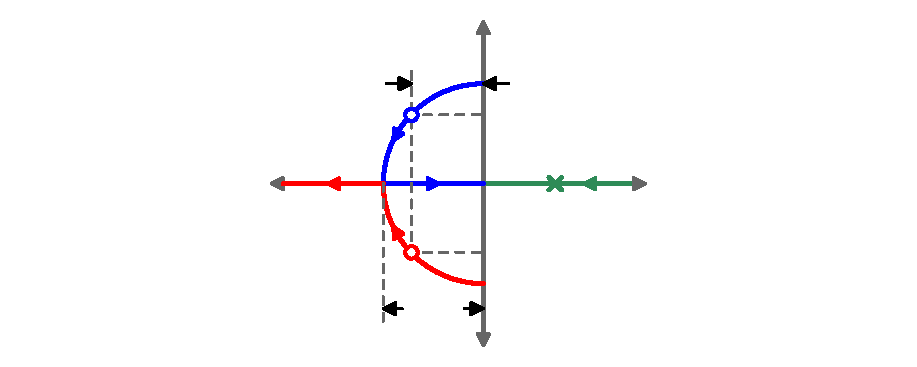
\includegraphics[scale=0.70000]{./figs/pi_pz_plot.pdf}\\
   % translate x=800 y=416 scale 0.38
   \putbox{2.85600in}{0.67900in}{1.20}{$\Re(s)$}%
   \putbox{2.30300in}{1.52600in}{1.20}{$\Im(s)$}%
   \putbox{1.89000in}{0.21700in}{1.20}{$\sqrt{\mathrm{K}}$}%
   \putbox{1.45600in}{1.36500in}{1.20}{$\zeta\sqrt{\mathrm{K}}$}%
   \putbox{2.38700in}{0.95900in}{1.20}{$\sqrt{\mathrm{K}}/2\zeta$}%
   } % close 'parbox'
   } % close 'scalebox'
   \vspace{-\baselineskip} % this is not necessary, but looks better
\fontfamily{\rmdefault}\selectfont

				\caption{PI-controller PLL pole-zero locations.}
				\label{fig:pi_pll_pz}
			\end{figure}
			\FloatBarrier
			To illustrate the effect of the damping coefficient $\zeta$, figure \ref{fig:pi_pll_response} illustrates the example frequency and step responses of a PI-controlled PLL with N=1. Notice excessive peaking and ringing for $\zeta<\sqrt{2}/2$. The peaking observed in the frequency response is unavoidable with the PI-PLL due to the inherent zero in the transfer function. Its effect can be reduced with large $\zeta$, however this will increase PLL settling time. 
			\begin{figure}[htb!]
				\center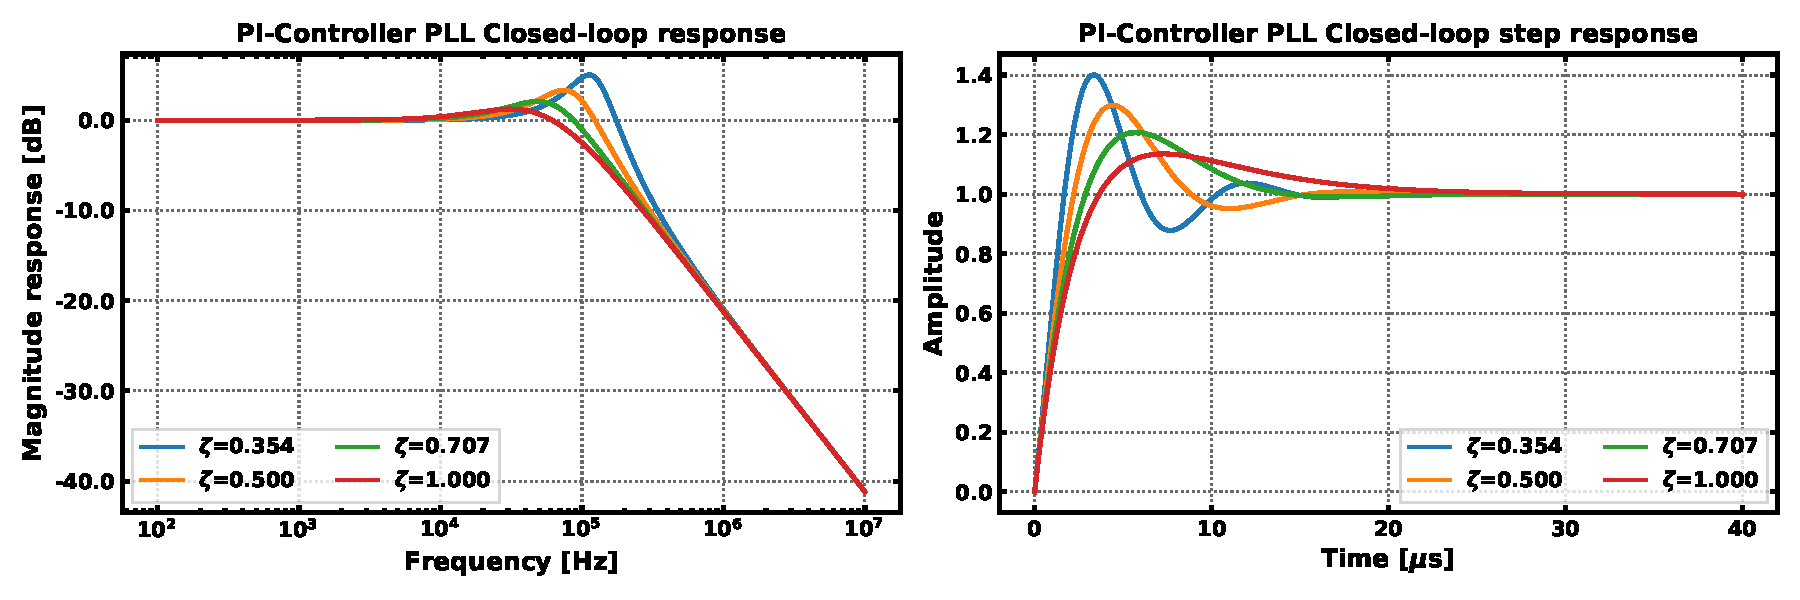
\includegraphics[width=1.0\textwidth, angle=0]{figs/pi_pll_response.pdf}
				\caption{Example PI-PLL responses with varied $\zeta$.}
				\label{fig:pi_pll_response}
			\end{figure}
			\FloatBarrier
			If $\zeta$ is constrained to $\leq 1$:
			\begin{equation}
				\tau = \frac{1}{|\min(\Re(\{s_{p1}, s_{p2}\}))|} = \frac{1}{\zeta\sqrt{K}}
			\end{equation}
			Thus:
			\begin{equation}
				t_s = \frac{-\ln(\delta)}{\zeta\sqrt{K}} = \frac{-\ln\left(\frac{f_{tol}}{|f_i - Nf_{ref}|}\right)}{\zeta\sqrt{K}} 
			\end{equation}
			Based on specification for settling time and damping $\zeta$, the values for K and $\omega_z$ can be determined. If $K_{VCO}$ and $\mathrm{N}$ are also specified, the PI gain coefficients can be solved additionally.
			\begin{align}
				\omega_z &= \frac{-\ln(\delta)}{2t_s} =  \frac{-\ln\left(\frac{f_{tol}}{|f_i - Nf_{ref}|}\right)}{2t_s}\\
				K &= \frac{\ln^2(\delta)}{\zeta^2t_s^2} =  \frac{\ln^2\left(\frac{f_{tol}}{|f_i - Nf_{ref}|}\right)}{\zeta^2t_s^2}\\
				K_i & = \frac{\mathrm{N}\mathrm{K}}{2\pi K_{VCO}} \\
				K_p & = \frac{K_i}{\omega_z}
			\end{align}

		\subsubsection{PI-controller peaking compensation}
			 To compensate for closed loop peaking, the original PI-controller loop filter of equation \ref{eq:pi_pll_tf} can be modified with the addition of a single tunable pole at $\omega_p$. The closed loop response becomes third order, which complicates direct analysis and design of the loop filter. However, utilizing the automated filter optimization approach described later in this paper resolved issues regarding filter design in this case.
			\begin{equation} \label{eq:pi_compensated_tf}
				\textnormal{H}_{LF}(s) = \frac{K_i}{s}\frac{\left(\frac{s}{\omega_z} + 1\right)}{\left(\frac{s}{\omega_p} + 1\right)}
			\end{equation}

		\subsubsection{Alternative PID controller permutations} \label{other_pid}
			If individual terms within the PID-controller are dropped, different controller permutations (PD, ID, PI, P, I, D) can be achieved. As mentioned before, inclusion of an integral term is needed to ensure the desired zero steady state error for a PLL. This leaves ID and I-controllers as possible alternative solutions to PI for the loop filter. It is shown in the following that neither of these controllers result in a stable PLL, which leaves a PI-controller as the only viable PID implementation.

			\textbf{I-only controller}

			Setting the $K_p$ and $K_d$ terms of equation \ref{eq:pid_pll_tf} to zero yields:
			\begin{equation}
				\frac{\Phi_{out}(s)}{\Phi_{ref}(s)} = \frac{2\pi K_{VCO}K_i}{s^2 + \frac{2\pi K_{VCO}}{\mathrm{N}}K_i}
			\end{equation}
			This closed loop transfer function results in a pair of poles at $\pm\sqrt{2\pi K_{VCO}K_i/\mathrm{N}}$. This will never be stable, as it can only be manifested as (1) a pair of poles on the imaginary axis, which is an oscillator, or (2) a real pole in the right-half plane and a real pole in the left-half plane, the former of which is not causally stable.

			\textbf{ID-controller}

			Setting the $K_p$ term of equation \ref{eq:pid_pll_tf} to zero yields:
			\begin{equation}
				\frac{\Phi_{out}(s)}{\Phi_{ref}(s)} = \frac{2\pi K_{VCO}\left(s^2K_d + K_i\right)}{s^2\left(1 + \frac{2\pi K_{VCO}K_d}{\mathrm{N}}\right) + \frac{2\pi K_{VCO}}{\mathrm{N}} K_i}
			\end{equation}
			The poles of this transfer have the same form as the I-only controller, and this PLL-controller configuration is unstable for the same reasons as the I-only controller PLL.